\documentclass[main.tex]{subfiles}
% \nomenclature[A]{GPR}{Ground Penetrating Radar}%

\begin{document}
\chapter{Conceptual Design}
\chaplabel{conceptDesign}
 \todo[inline]{maybe: "The conceptual design presents the design requirements......." - HV}
This chapter presents the design requirements and concept solutions for the various project subsystems, namely the sensor subsystem, including signal processing and sensor fusion, the platform subsystem, including automation and navigation, and the sensor mount subsystem. \textcolor{red}{\textbf{General comments for conceptual design: Quantify requirements in detail and use the info developed in the feasibility study to make a decision about the component to select}}


\section{Sensor selection}
\todo[inline]{As maz said, did we select the sensors or had we already 'chosen' them before the project started, feasibility study only mentions MD and GPR so maybe we had already chosen them before the project. maybe rename this section to "Sensor Background", or "Sensor Introduction" or "Sensor Description" or just get rid of it entirely? - HV}
The selection of sensors for the project was based on the requirements from the scenario of operation. These are as follows: \textcolor{red}{Maz: need numbers for these requirements}

\begin{itemize}
\item Detection of various target types: The sensor suite should be able to detect anti-personnel and anti-tank mines with high and low metal content 
\item Detection speed and depth: The sensors must be capable of real time detection at an operational speed of 5 km/h and depths of up to 15 cm
\item Accurate discrimination: The chosen sensors must be able to discriminate between landmines and other objects, with the aim to minimise false positives
\end{itemize}

As outlined in the benchmarking section, the primary sensors used for landmine detection operations are metal detectors and GPRs. When used in isolation, each sensor has several limitations. Metal detectors can only be used to detect metallic mines, they produce a large number of false positives, and their penetration depth is restricted. On the other hand, GPR systems produce data that is difficult to interpret, and is also very sensitive to environmental conditions such as soil type and moisture content. In both cases, signal processing of some form is required, either using software to identify detected objects, or with the involvement of a skilled operator.

Multisensor systems allow a greater range of targets to be identified. In addition, having two sensors provides the ability to confirm the presence of metallic mines, which reduces false positives and thereby increases the efficiency of operations. While it is difficult to quantify this increase in efficiency, this result has been demonstrated in experimental work carried out by \textcite{Takahashi10}. As can be seen in \Figref{FAR}, the false alarm rate, defined as the number of false alarms per unit area, for a system that combines a metal detector and GPR is roughly half that of a metal detector alone. Thus, a multisensor system meets the necessary requirements outlined above, while addressing some limitations of individual sensor systems. \textcolor{red}{\textbf{General comment for all figures: shows/label items in figure (post-process), make sure font size is at least as large as the text, assume it will be in black and white (i.e. don't refer to colours in the figure, number or label things instead)}}

\begin{figure}[ht]
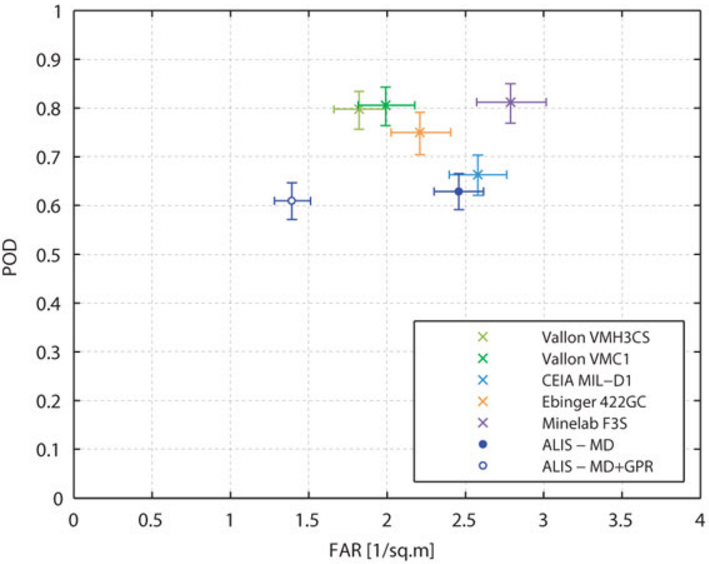
\includegraphics[width=0.6\textwidth]{3-ConceptDesign/FAR.PNG}
\centering
\caption[Reduction in false alarm rate as a result of using a multisensor system]{Reduction in false alarm rate observed as a result of using a multisensor system (ALIS-MD+GPR) as opposed to a metal detector alone \parencite{Takahashi10}} \figlabel{FAR}
\end{figure}

Initially, it was expected that the sensor suite would be comprised of a metal detector array and a GPR array provided by the DSTG, with a total payload weight of 80 kg. The use of the 3 m wide arrays would allow for larger areas to be scanned in a shorter period of time, leading to an increase in operational efficiency. Due to unforeseen circumstances, the arrays could not be made available for the project, and so smaller line scan sensors had to be used instead. Off-the-shelf sensors were then considered, however most were not able to produce any raw data output that could be processed to meet the project objectives. In the case of GPR systems, the high cost of systems was also a limiting factor. Eventually, a pair of sensors were borrowed from the DSTG, the specifications of which are presented below. Despite the fact that line scan sensors were used, it was assumed that the scanning arrays would be made available by the completion of the project, and so the size and weight specifications of the arrays were used in selecting the platform and designing the sensor suite. 

\subsection{AMDS metal detector panel}
\todo[inline]{again, this isnt conceptual design, just information on the sensor we will be using}
The AMDS is a metal detector panel produced by Minelab (\Figref{AMDS}). The device has three sets of transmitting coils and a single receiving coil, allowing for three channels of data to be recorded at once. Each channel operates at four frequencies, 1.5 kHz, 4.5 kHz, 13.5 kHz and 40.5 kHz, which means that in total up to 12 sets of data can be recorded simultaneously. This recorded data contains the real and imaginary parts of the voltage signal measured due to changes in magnetic flux in the target. The data is transferred to a computer through USB, where it can be seen in real-time using a LabVIEW virtual instrument called Dataspleen, or saved in CSV format. The metal detector requires a 10 volt power supply at 0.5 amps.  

\begin{figure}[ht]
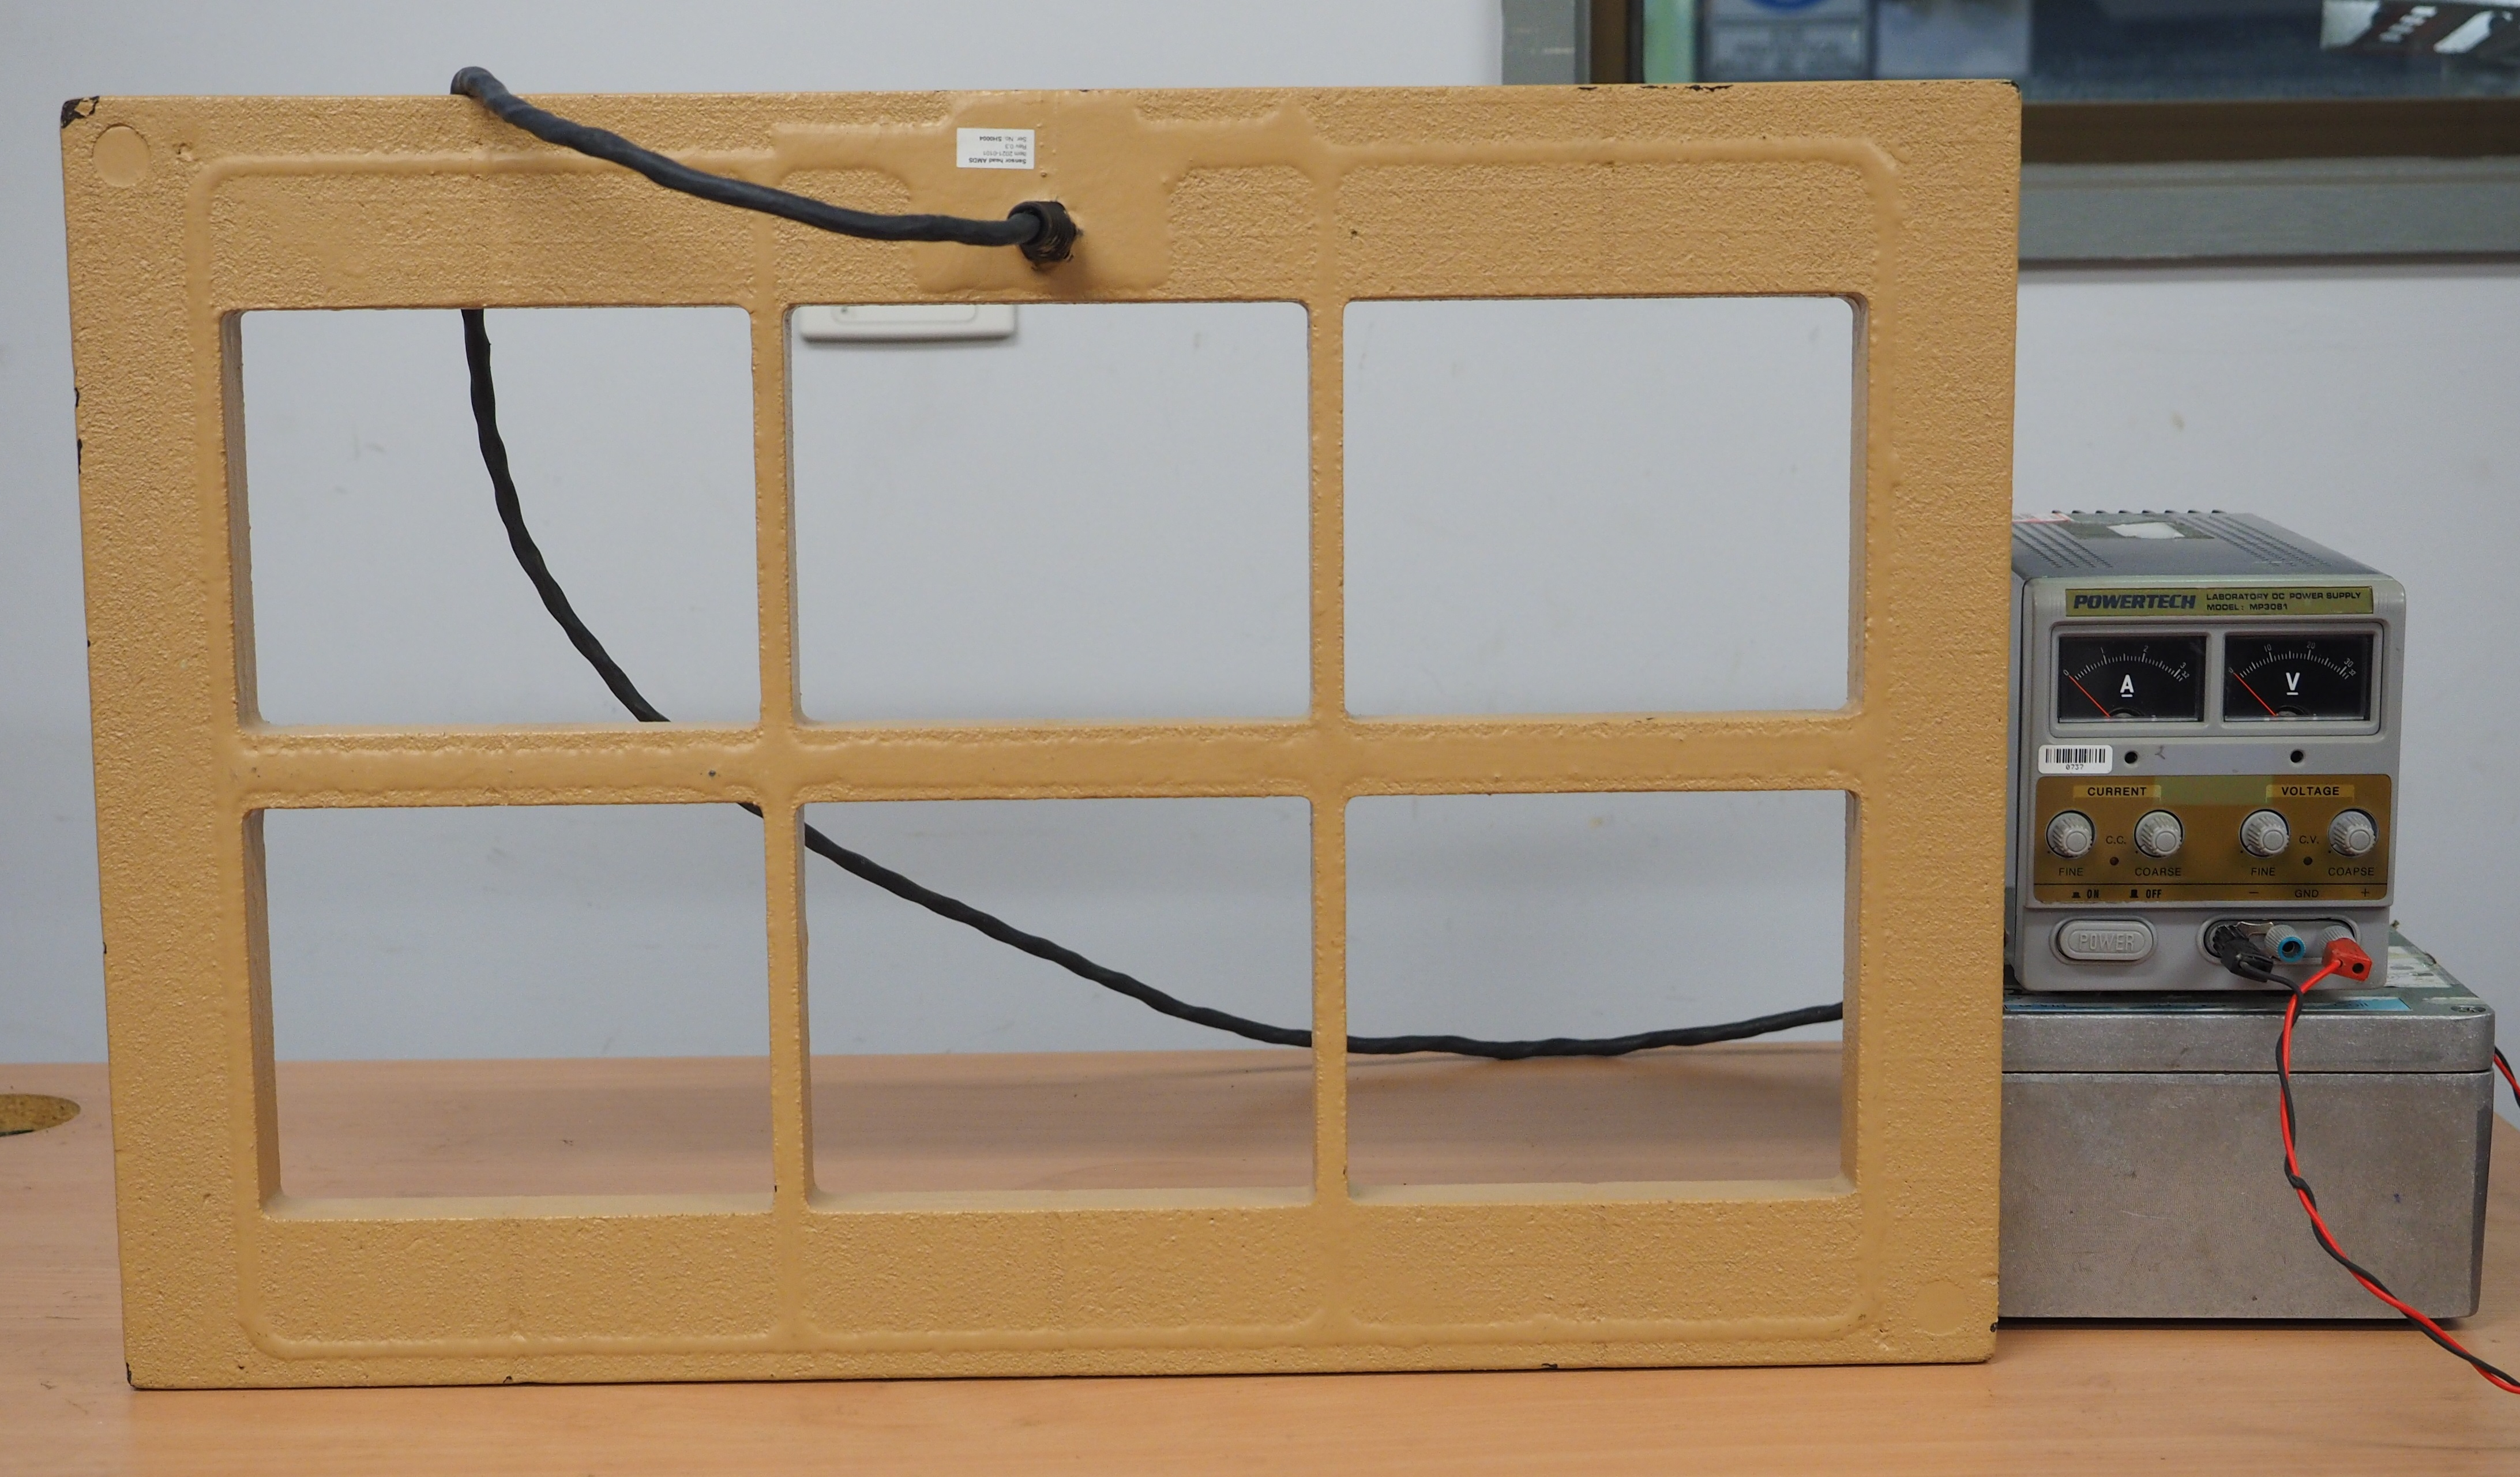
\includegraphics[width=0.5\textwidth]{3-ConceptDesign/AMDS.JPG}
\centering
\caption{AMDS metal detector panel with power supply and control unit} \figlabel{AMDS}
\end{figure}

\subsection{SIRO-PULSE II GPR unit}
The SIRO-PULSE II is a handheld GPR unit developed by the CSIRO, originally intended for the inspection of buildings (\Figref{siro}). It is a pulsed radar that can operate in either bi-static or differential antenna configurations, producing three sets of data in total. The unit comes with three interchangeable antenna heads of frequencies 800 MHz, 1.4 GHz and 2 GHz, allowing the resolution and penetration characteristics of the radar to be varied. Data is transferred to a computer via USB, where it can be viewed in real-time with the accompanying SiroPuleII software program. The program produces outputs of the frequency waveform over time, which are collected together to produce a B-scan in real time. The unit is battery powered with a runtime of up to 10 hours. 

\begin{figure}[ht]
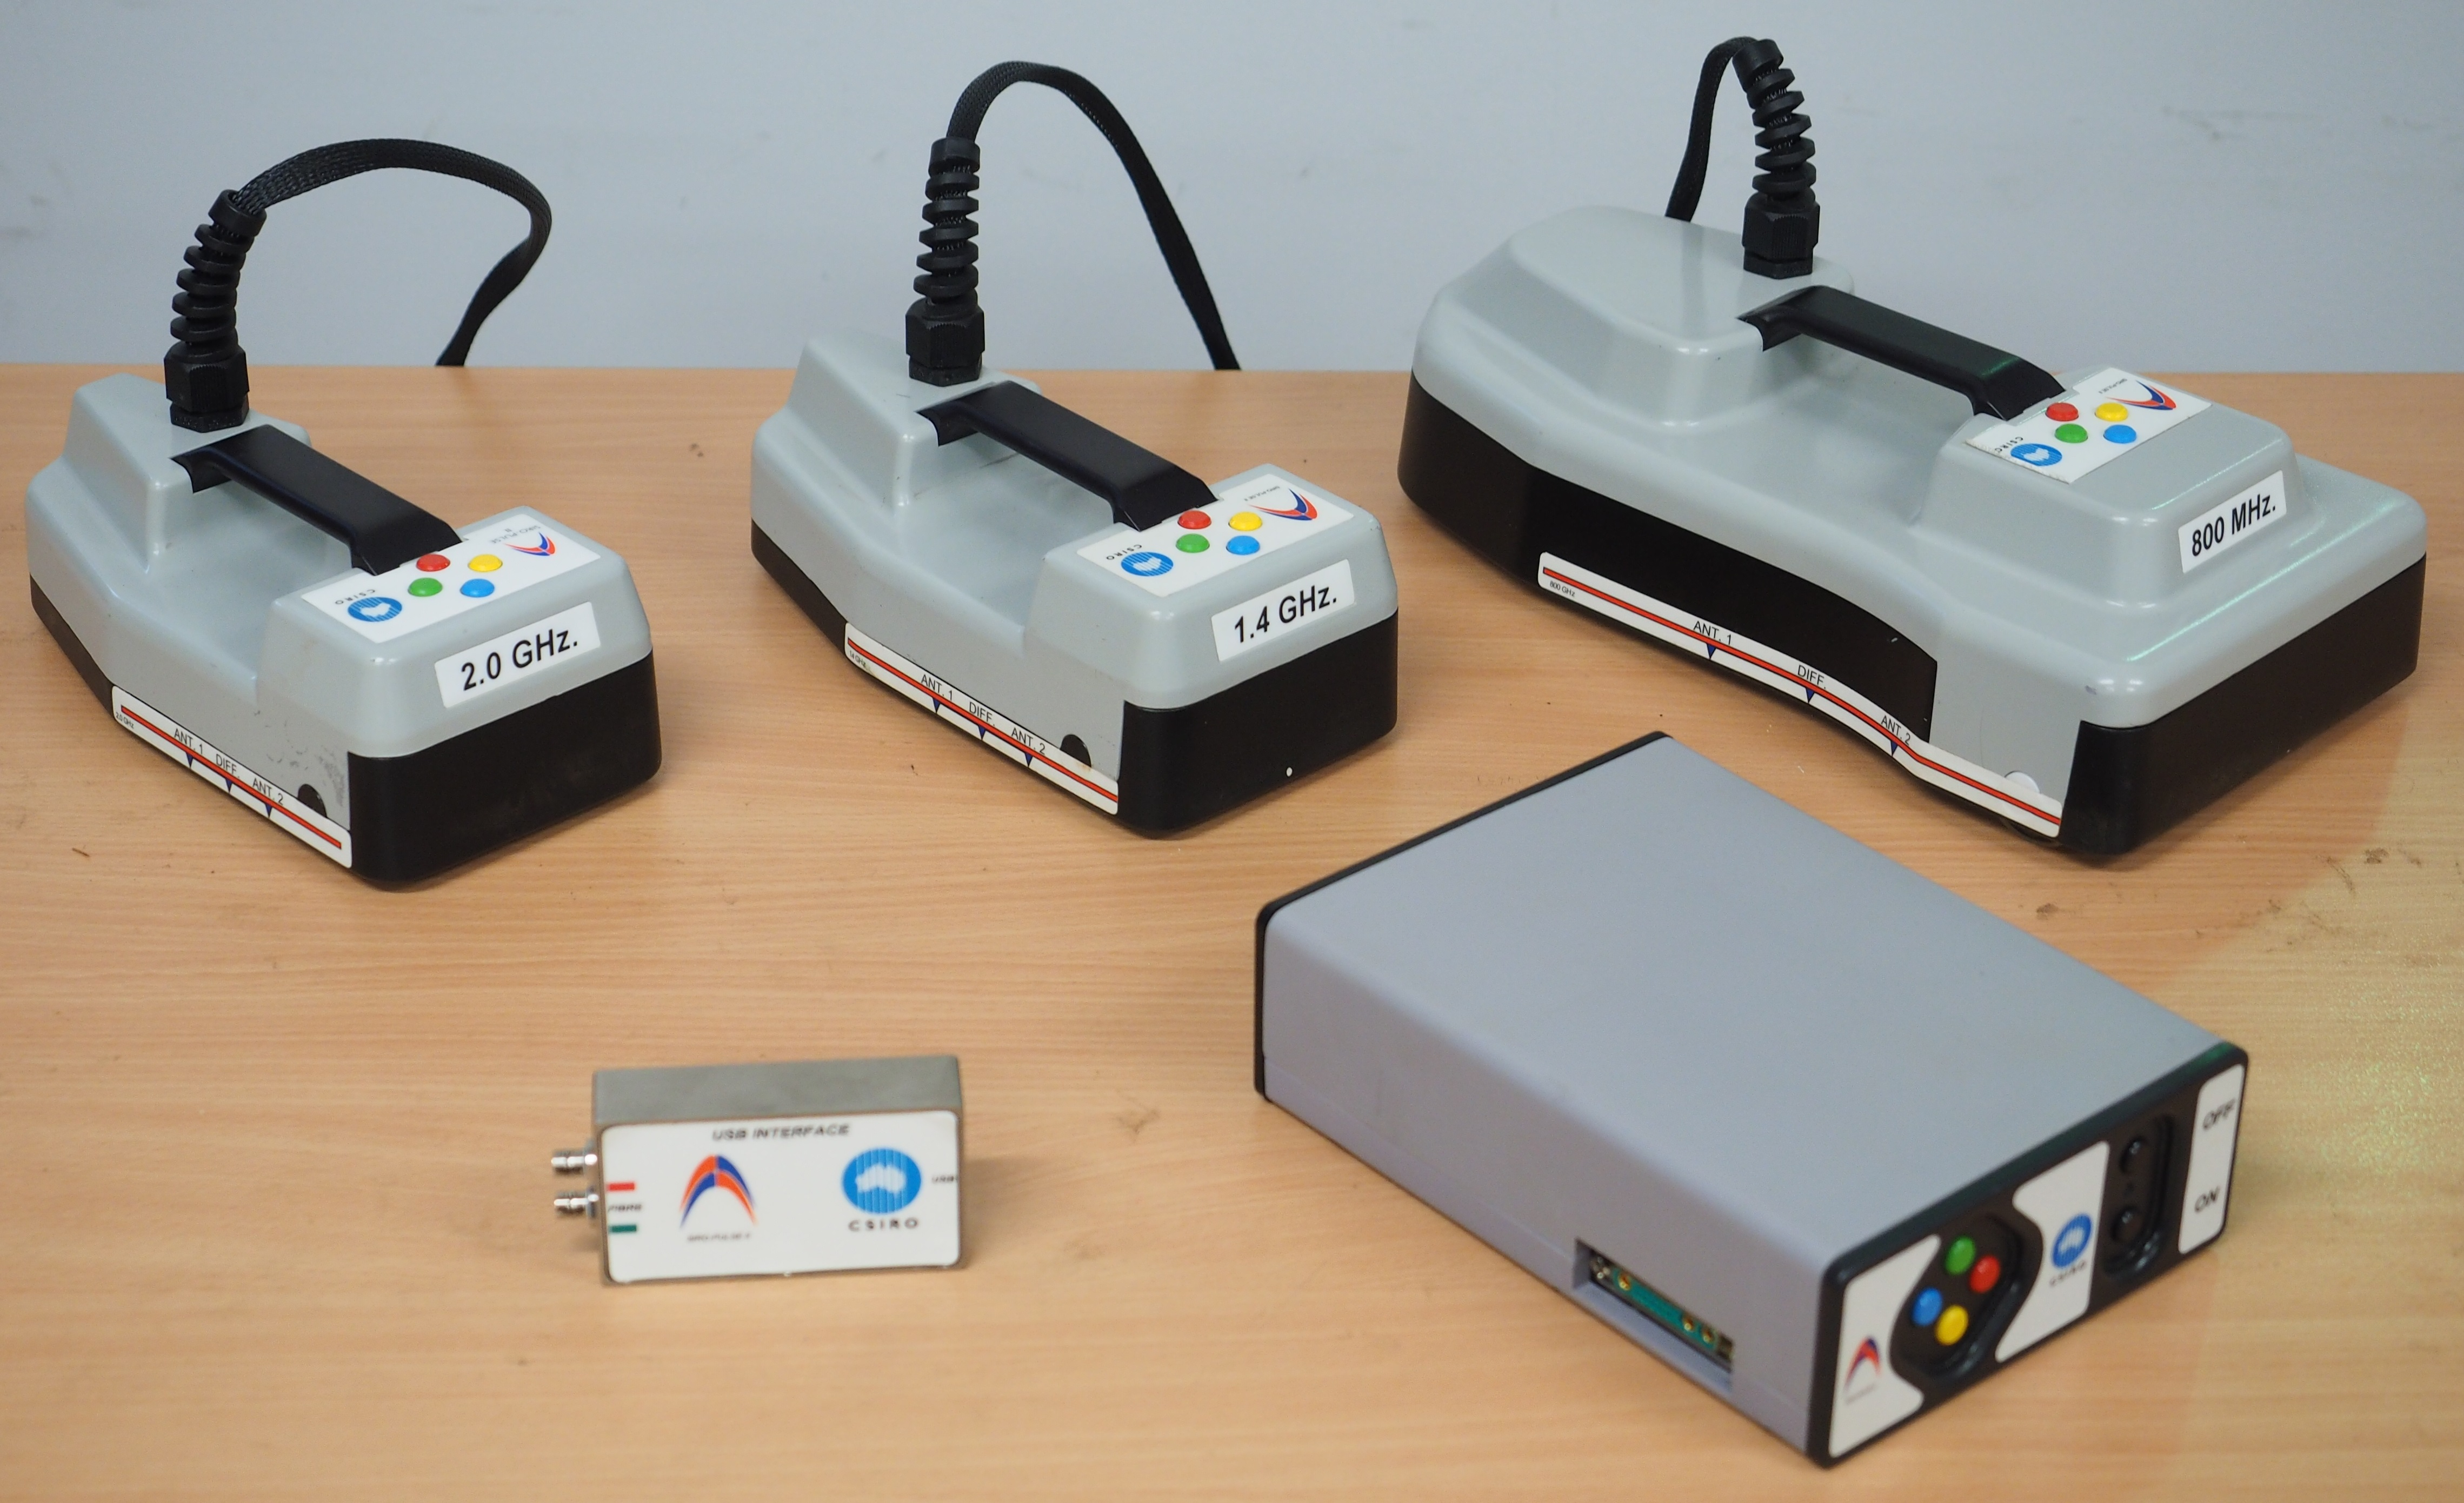
\includegraphics[width=0.5\textwidth]{3-ConceptDesign/SiroPulse.JPG}
\centering
\caption{SIRO-PULSE II GPR unit with control unit and antenna heads} \figlabel{siro}
\end{figure}

\section{Sensor fusion and signal processing}
\seclabel{signalConcept}
Regardless of the fact that the sensors suite met the outlined requirements, there were several key challenges to be addressed, namely sensor fusion and signal processing. The first of these relates to how the data from the separate sensors can be consolidated to provide a single meaningful result, while the second involves processing the output from the sensors to allow an operator to identify targets. 

\subsection{Sensor fusion}
As discussed in the literature review, there are three primary levels of sensor fusion, decision level, feature level and data level \parencite{Yarovoy2009}. Of these, decision level sensor fusion was selected as it offers the simplest and least computationally intensive solution, since the outputs from the sensors can be processed individually. This method also lends itself well to machine learning techniques, allowing a target to be identified based on correlations with a known dataset. The main disadvantage of this method is that it is not as robust as the other methods, however this was not expected to be an issue given the scope of the project. 

To be able to implement decision level sensor fusion, a decision needs to be made with each sensor regarding whether or not the target is a mine. This decision, along with a confidence interval, can be passed onto the sensor fusion algorithm as shown in \Figref{fusion}, which assigns then makes the final decision based on a weighted evaluation of the data it has received. In order for each sensor to make a decision, metrics need to be identified which can be used to characterise targets. As a result, preliminary tests were carried with both sets of sensors to find such metrics.

\begin{figure}[ht]
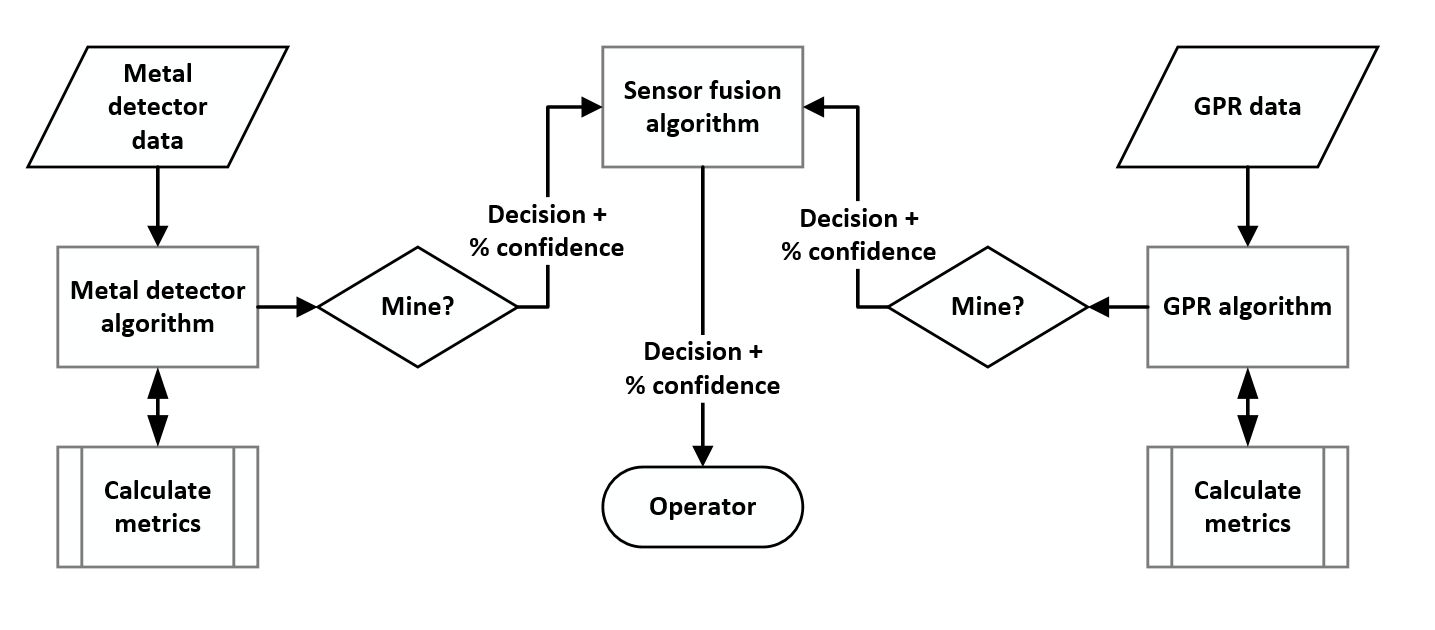
\includegraphics[width=0.85\textwidth]{3-ConceptDesign/fusion.PNG}
\centering
\caption{Integration of signal processing and sensor fusion algorithms} \figlabel{fusion}
\end{figure}

\subsection{Metal detector output}
Initial tests with the metal detector were performed indoors. In the first set of tests, horizontal sweeps were made over a number of small metal samples (\Figref{samples}) placed on the floor, with the distance to the metal detector being kept constant at 32 cm. 

\begin{figure}[ht]
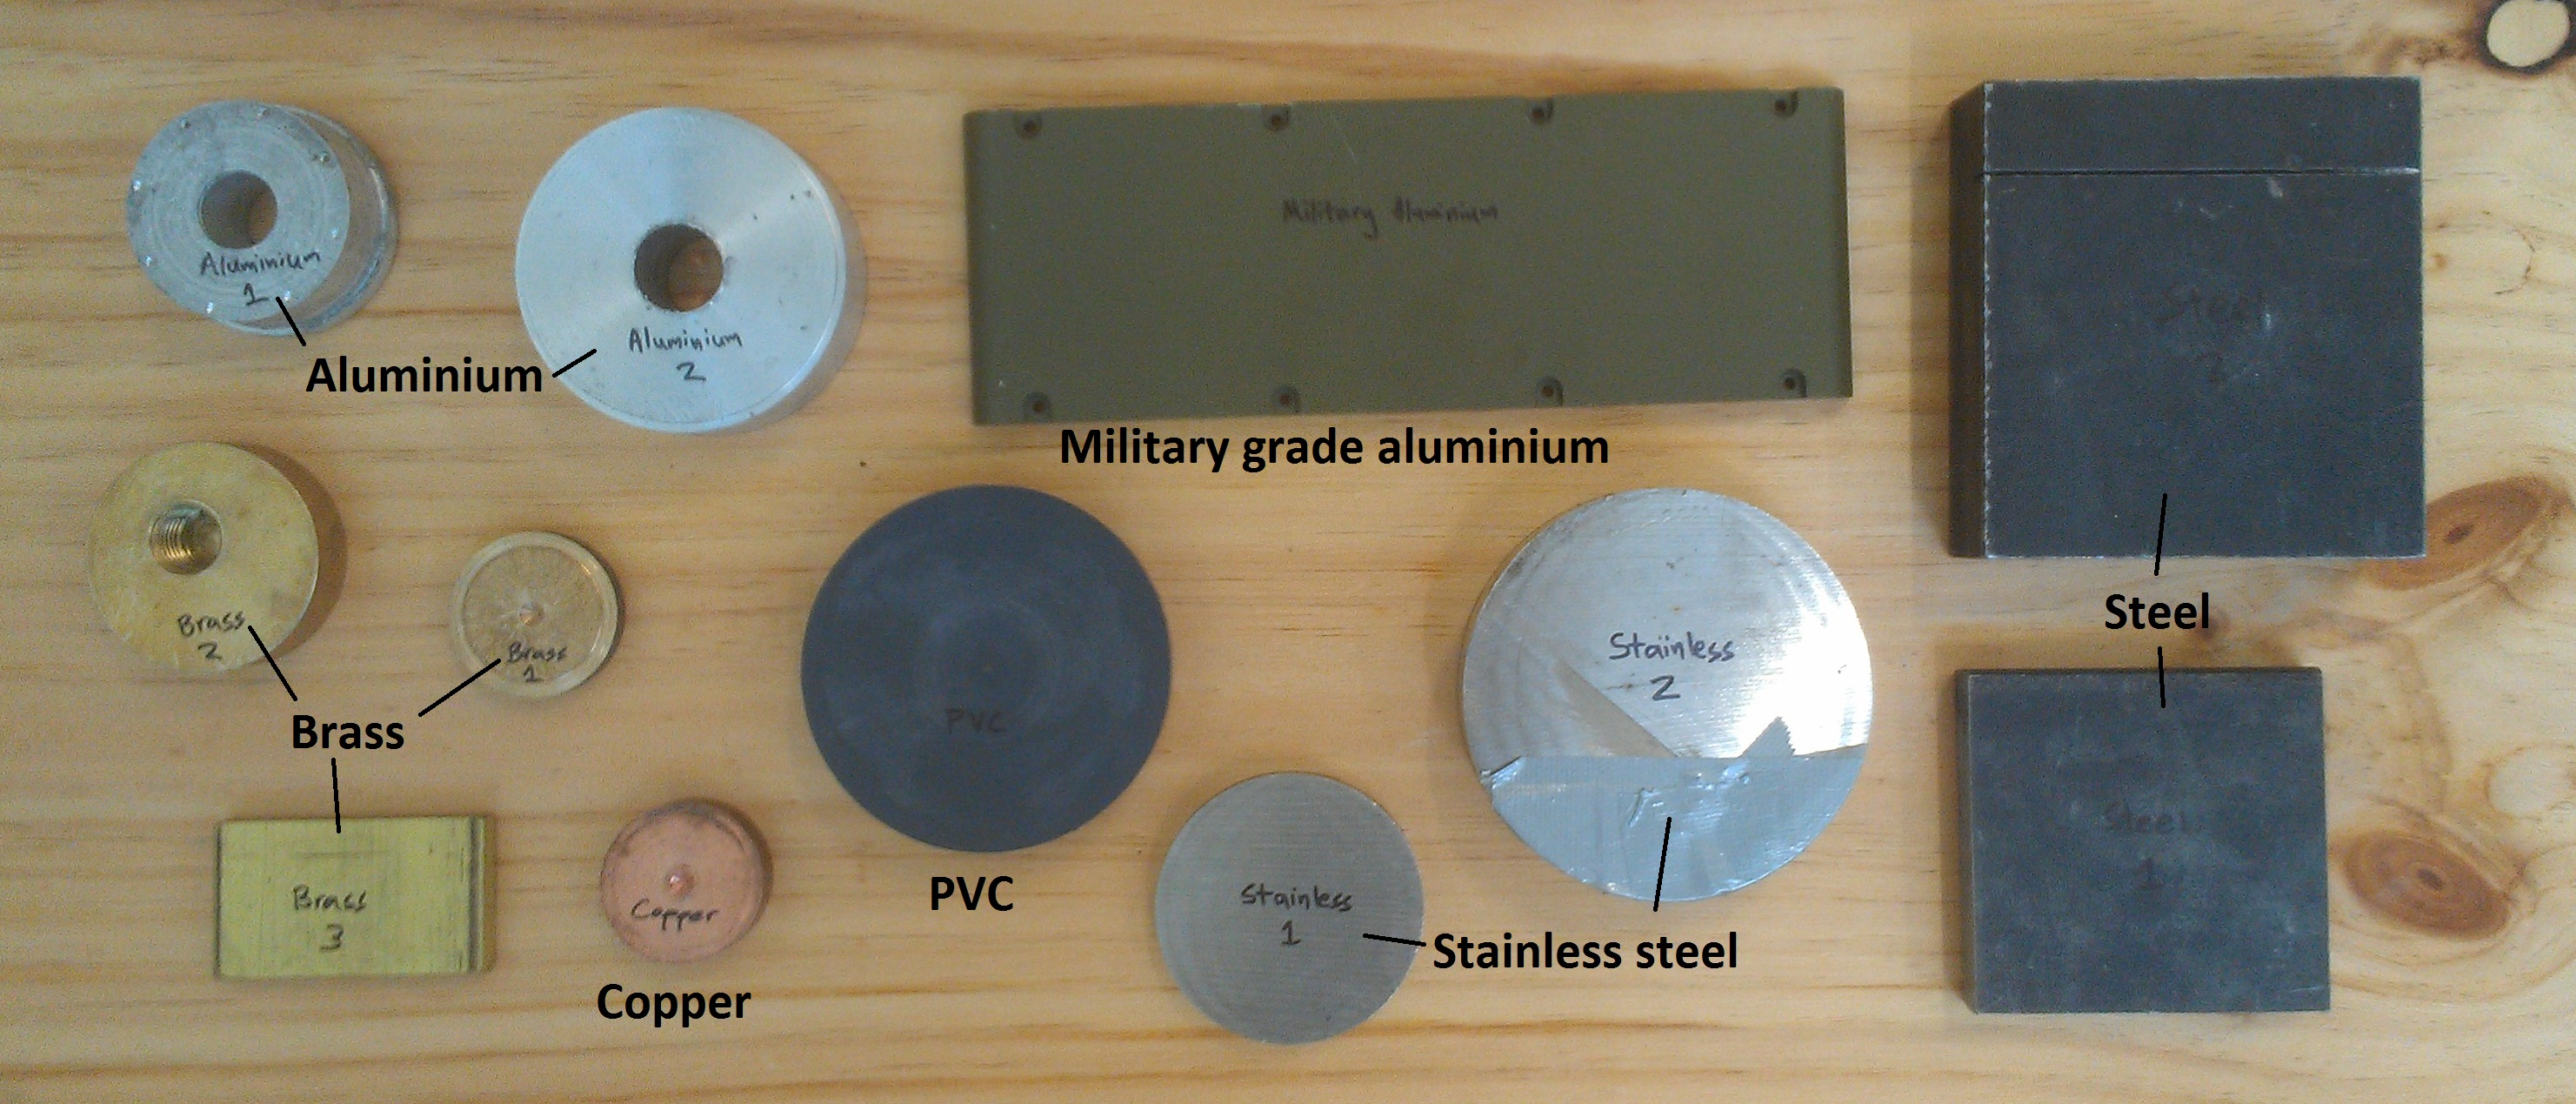
\includegraphics[width=0.8\textwidth]{3-ConceptDesign/samples.jpg}
\centering
\caption{Metal samples used for evaluation of metal detector outputs} \figlabel{samples}
\end{figure}

\Figref{metals} shows the results obtained from the second channel plotted in Matlab. The four lines in each plot correspond to the four frequency signals, while the axes represent the real and imaginary components of the voltage signal. It can be seen that for different metals, the magnitude and phase angle of the signal vary, as discussed in the literature review. 

\begin{figure}[ht]
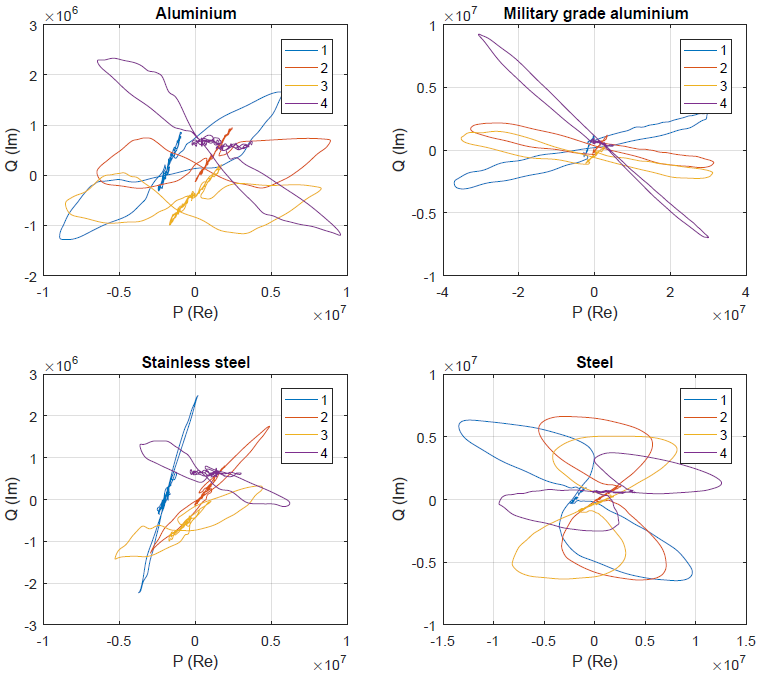
\includegraphics[width=0.65\textwidth]{3-ConceptDesign/metals.PNG}
\centering
\caption{Phase plots for several different metal samples at 32 cm depth} \figlabel{metals}
\end{figure}

In the second set of tests, a single brass sample was scanned, with the distance to the metal detector changed between scans. The results are shown in \Figref{phaseDepths}, and while the phase angle does not vary with depth, the signal magnitude does. Based on on these tests, it was concluded that the magnitude and phase angle of the signal would be suitable metrics for characterising objects; the phase angle can be used to identify the metal, while the magnitude provides information about the depth, size and material. Thus, the aim of the signal processing algorithm for the metal detector is to find these metrics given the metal detector input data. 

\begin{figure}[ht]
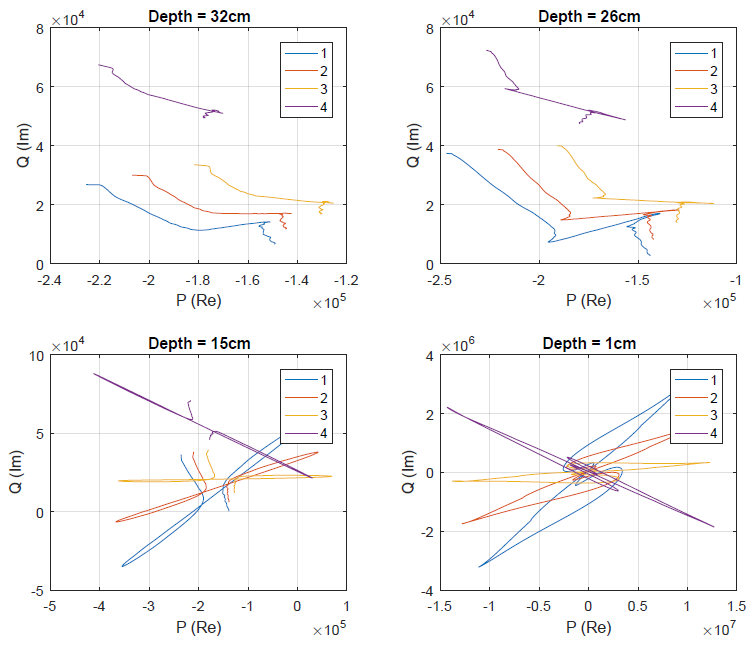
\includegraphics[width=0.65\textwidth]{3-ConceptDesign/phaseDepth.PNG}
\centering
\caption{Phase plots for a brass sample scanned at different depths} \figlabel{phaseDepths}
\end{figure}

\subsection{GPR output}
Preliminary tests for the GPR could not be conducted at the same time as metal detector testing due to issues in operating the GPR. However, sample datasets were provided by the DSTG, and these were analysed in Matlab. \Figref{cans} shows the B-scans for an empty (background) scan, as well as a scan over two soft drink cans. 

Unlike with the phase plots obtained from the metal detector, it was not as clear what metrics could be identified from the GPR data. To further aid in visualising the signal, the background was subtracted (\Figref{cansNoBG}). This made it easier to identify features in the scan, the size and position of which could be found easily. Once the position of the feature is known, the A-scan corresponding to the feature can be extracted, and this can also be used to characterise the feature. Hence, the chosen metrics for the GPR are feature size, feature position and A-scan characteristics.

\begin{figure}[ht]
\centerline{
\begin{tabular}{cc}
\subfloat[]{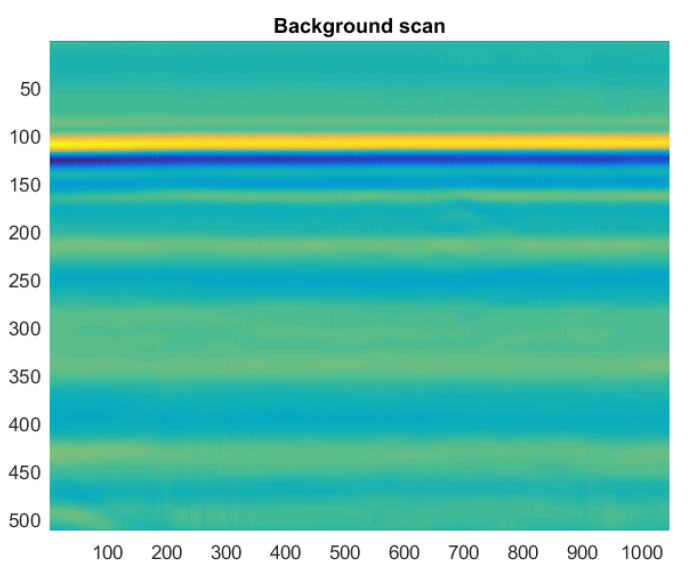
\includegraphics[width=0.47\textwidth]{3-ConceptDesign/bg.PNG}}
& \subfloat[]{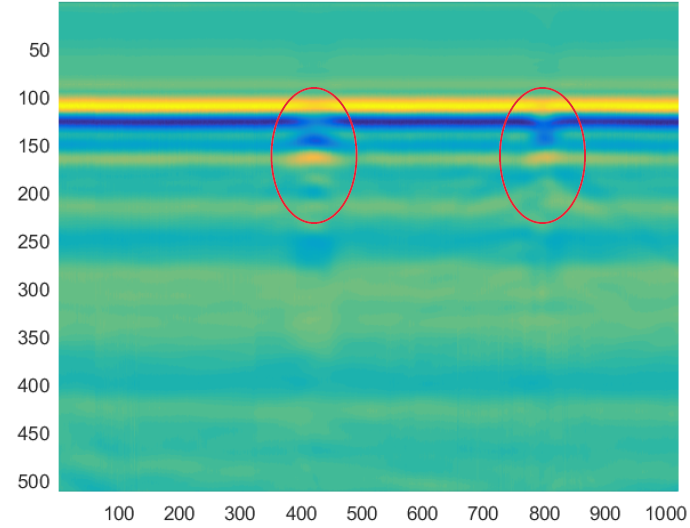
\includegraphics[width=0.47\textwidth]{3-ConceptDesign/cans.PNG}}\\
\end{tabular}}
\caption[Background scan over two soft drink cans]{Background scan (a) and B-scan over two soft drink cans, circled in red (b)} 
\figlabel{cans}
\end{figure}

\begin{figure}[!ht]
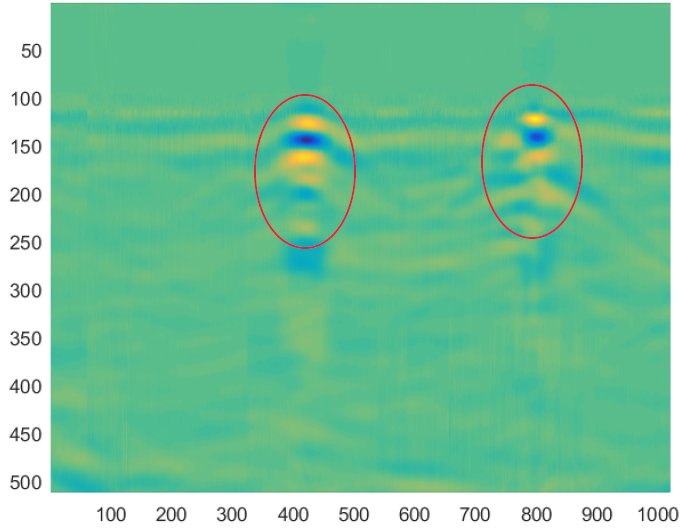
\includegraphics[width=0.6\textwidth]{3-ConceptDesign/cansNoBG.PNG}
\centering
\caption{B-scan for soft drink cans with background removed} \figlabel{cansNoBG}
\end{figure}

\section{Platform selection}
\seclabel{platformselect}
The platform is used to mount the required detection equipment and acts as the foundation for a completely autonomous system. The design and construction of a new platform was considered to be outside the scope of the project, and so the modification of an existing platform was the preferred approach. The requirements for the platform primarily come from the scenario of operation, but also include some other considerations: 

\begin{itemize}
 \item Payload: The platform should be able to carry a total payload of 100 kg, and must allow for this payload to be mounted.
 \item Terrain traversing: The platform should be able to travel off-road in regions with dry sandy soils and level unobstructed terrain.
\item  Operational speed and acceleration: The platform should be able travel in a straight line, both forwards and reverse, and perform turns while maintaining an operational speed of 5 km/h.
\item Manoeuvrability and controllability: The platform should be manoeuvrable enough to navigate a region of interest, with a smaller turning angle preferred, yet controllable enough that in case of an emergency, it can come to a complete stop from its operational speed in 1 m.
\item Cost and availability: The platform should have a reasonable cost given the project budget of \$16,500, ans should be available for use as early as possible. 
\item Ease of automation: The platform should be sufficiently simple to automate, with a preference given to platforms that have the framework for automation already implemented. 
\item Ease of transportation: The platform should be sufficiently easy to transport from a workshop to a testing locations using a ute or trailer.
\end{itemize}

The detailed platform selection process is outlined in \Chapref{platformSelectionApp}. Several platforms were considered and evaluated against the above requirements, and the most appropriate platform was found to be an autonomous quad bike provided by the DSTG (\Figref{quadbike}). The quad bike is a Honda TRX450r, and was previously modified at the University of Adelaide on several occasions, most recently by \textcite{scheiner2011}. 

\begin{figure}[ht]
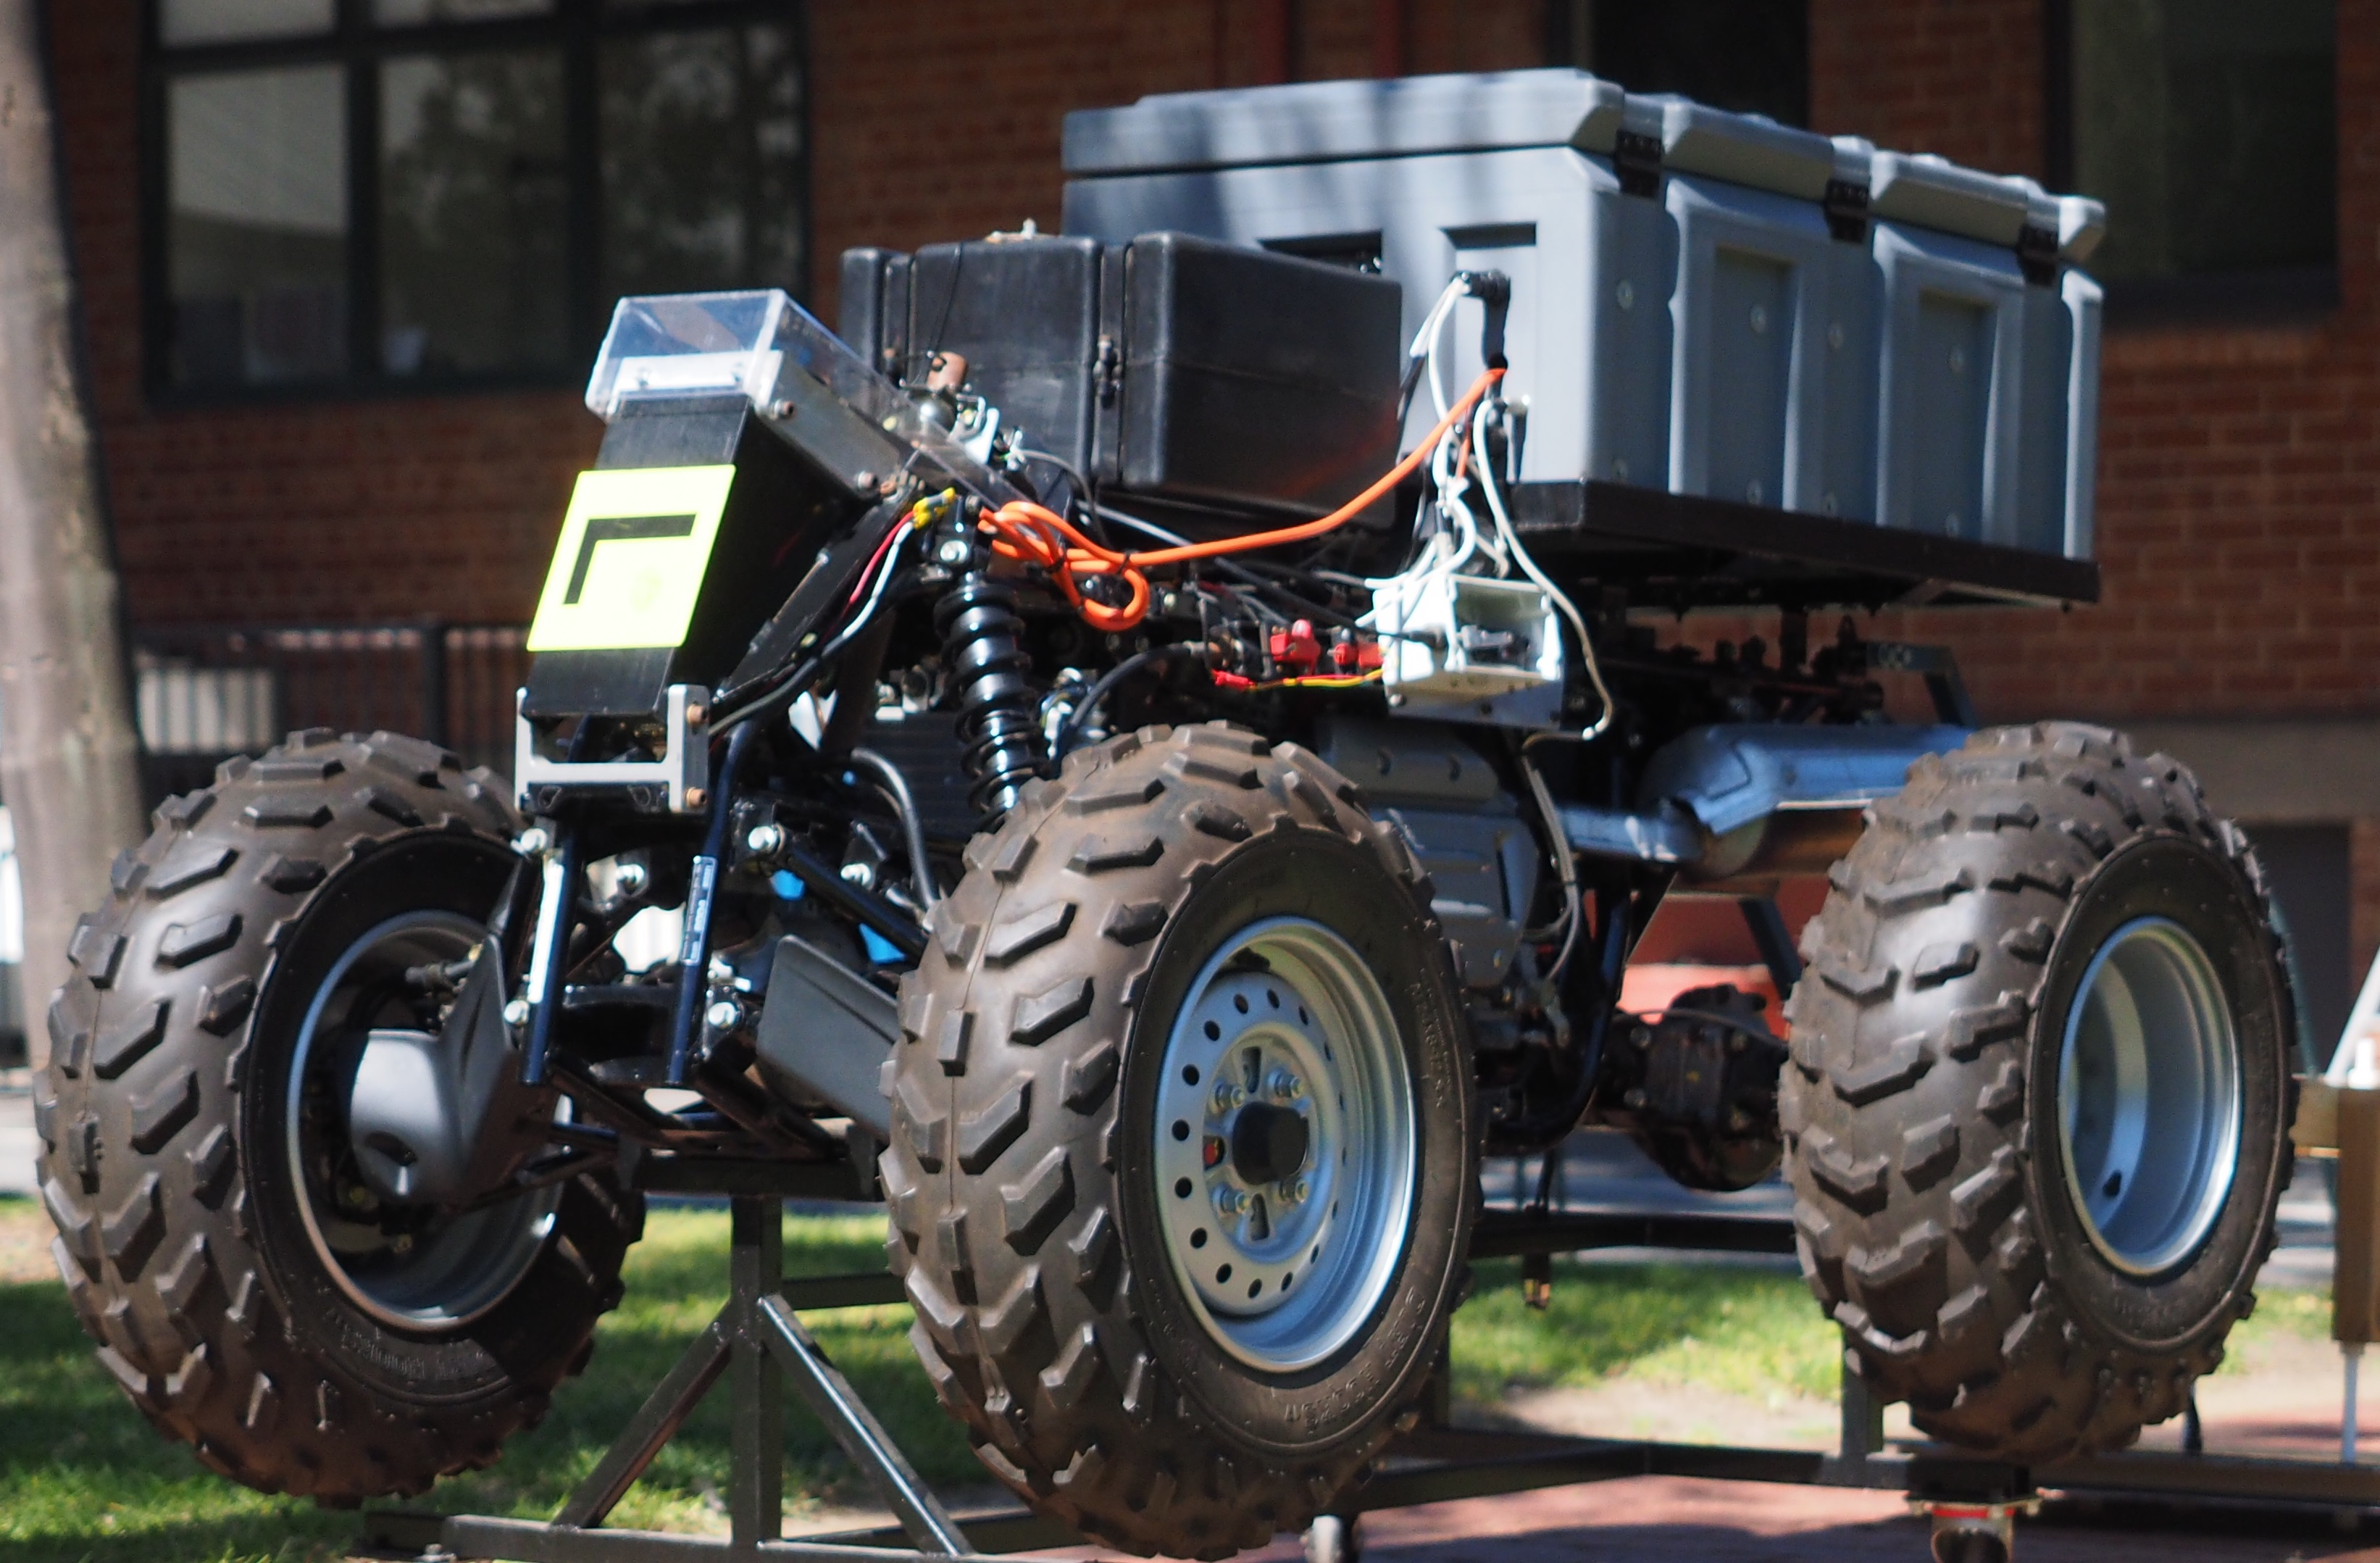
\includegraphics[width=0.6\textwidth]{3-ConceptDesign/bike.JPG}
\centering
\caption{DSTG autonomous quad bike} \figlabel{quadbike}
\end{figure}

The intended application for the quad bike was to autonomously drive through vineyards. In order to achieve this, a number of systems had to be modified, namely the steering, throttle, brake and gear change systems \parencite{scheiner2011}. The steering is controlled by an Animatics Smart Motor, connected to the steering column using a v-belt. A servo motor is to control the throttle, while a wheel speed encoder measures the vehicle's position. The linear actuator is used to control the brakes, with a strain gauge used to measure the braking intensity. Finally, two linear potentiometers are used to measure the position of a linear actuator in the gear system. A Dragon Board is used as the main controller, handling communications between all subsystems. 

\section{Automation and navigation}
The navigation and automation systems are responsible for instructing the quad bike as to what path it should follow, which is achieved through the control of the various actuators. As stated in the scenario of operation, platform navigation will be primarily handled using waypoints. At the start of a mission, the operator will select waypoints that define either a path, or the boundaries of some region of interest. If a region is selected, it is broken down into a series of waypoints which, once connected, will form a path for the quad bike. In the alternate use case, the navigation system will operate based directly on waypoints created from a user defined path.

\subsection{Path tracking}
\seclabel{pathconcept}
As the platform will be primarily performing two tasks, following a low curvature curve (straight line) and turning a specified angle, the navigation system will define the path using a 'piecewise linear path' discussed in \secref{pathTrackingLitReview}. \Textcite{snider2009} provides an empirical comparison of path following algorithms, shown in \Figref{trackingComparison}. Tracking methods are ranked by implementation difficulty, from least difficult to most difficult. \Textcite{snider2009} goes on to describe recommended applications for each method. Pure Pursuit is ideal in situations for slow driving and/or on discontinuous paths, the Stanley method for smooth highway driving and/or parking manoeuvres, the Kinematic model for smooth parking manoeuvres, and the Dynamic model for highway driving at speed. Based on the scenario of operation, which involves slow driving on discontinuous paths, the Pure Pursuit method is the most appropriate option, and will be used as the tracking method.
\begin{figure}[ht]
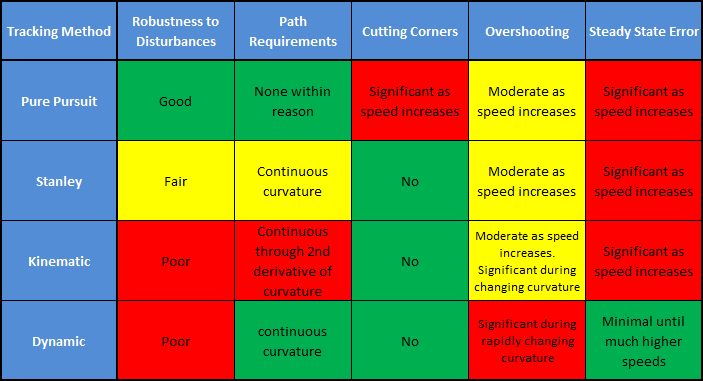
\includegraphics[width = \textwidth]{3-ConceptDesign/pathTrackingSummary2.png}
\centering
\caption[Empirical comparison of path tracking algorithms]{Empirical comparison of path tracking algorithms \parencite{snider2009}} \figlabel{trackingComparison}
\end{figure}

\subsection{Performing turning manoeuvres}
During scanning of an area, whenever the platform reaches a boundary, it will be required to turn some specified angle within a small area defined by the width of the 3 m sensor arrays. This prevents the platform from travelling over unscanned areas and potentially detonating a landmine. Alternatively, if the scan history for the surrounding region is available to the platform in the form of a map, a larger area may be available to conduct the turn. Due to there being little or no literature available on this unique topic, an adaptation of the simplified Ackermann model will be used in conjunction with the Stanley model, which excels for parking manoeuvres \parencite{snider2009}, to achieve the desired turn.

\subsection{Positioning}
The positioning system is used to determine the location of the quad bike for navigation, and to send that data to the operator's handheld device when a landmine is detected. Real time positioning in remote locations and accuracy to within 0.5 m is required from the system to meet the needs of the scenario of operation. A number of options were looked at when designing the positioning system including Local Positioning Systems (LPS), Global Positioning Systems (GPS), and dead reckoning techniques.
\nomenclature[A]{GPS}{Global Positioning System}%
\nomenclature[A]{LPS}{Local Positioning System}%

LPS use three or more signalling beacons of known location to determine a position through triangulation. These systems can be highly accurate, however they require the signalling beacons to be stationed near the area of interest. Transporting and setting up at least three signalling beacons is a time consuming process and is particularly inefficient when numerous areas of interest are required to be scanned. Since personnel are needed to place the beacons in potentially dangerous area, this method was not considered any further. 

Similar to LPS, GPS measurements are very accurate. However, due to the distance between receivers and a number of linked effects, the positional data is very noisy, providing location reliably within only 4 metres. Better accuracy can be achieved by using correction techniques, such as Real Time Kinematics (RTK), which can provide sub-centimetre accuracy. Similar to LPS, correction methods like RTK require base locations within 15 kilometres of the GPS and can take many seconds to receive a fix, both of which make it difficult to achieve real time positioning in remote areas.
\nomenclature[A]{RTK}{Real Time Kinematics}%

Dead reckoning techniques calculate the current position by advancing a previous position, based on a known speed and heading over some time step. These techniques are highly prone to cumulative error known as drift. A widely used application of dead reckoning is in Inertial Measurement Units (IMU), where accelerometers and gyroscopes are used to determine linear and rotational accelerations and thus have information to update position. This method is able to provide positional data in real time, however over longer time periods the accuracy becomes unreliable.
\nomenclature[A]{IMU}{Inertial Measurement Unit}%

To correct for drift from dead reckoning techniques, GPS aided Inertial Navigation Systems (INS) can be used. Accurate but noisy data from a GPS is constantly fed into an estimation algorithm alongside a smooth, but error accumulating position to correct for the drift. Kalman Filtering is one such technique which is used to combine information from various sensors to provide a much more reliable estimate of position.
\nomenclature[A]{INS}{Inertial Navigation System}%

\section{Sensor mount}
\seclabel{sensormount}
The sensor mount is required to support the weight of both the GPR and the metal detector, while being sturdy enough to isolate the sensors from vibrations caused by the platform. The following section describes the requirements imposed on the mount, the selection of appropriate materials and mounting location on the quad bike, as well as initial designs.  

\subsection {Sensor requirements} 
The design of the mount must satisfy two operating requirements for each sensor, the maximum operating height above the ground and the minimum proximity to other objects to prevent interference. 

Sensitivity tests with the AMDS metal detector panel found that metal objects at distances greater than 35 cm could not be detected, regardless of material or size. Based on this, a minimum proximity of 40 cm was specified. To maximise sensing depth, the metal detector should be placed as close to the ground as possible. However, resting the detector on the ground may result in damage if the platform vibrates excessively, or a small obstacle is encountered. Taking this into account, a maximum ground clearance of 5 cm was specified.

Tests were also carried out with the SIRO-PULSE II GPR unit, resulting in negligible interference from nearby all objects. Thus, a minimum proximity was not specified for the GPR. In order to reduce the effect of the air-ground interface and other sources of interference, the GPR should operate as close to the ground as possible. If the wheel encoder on the GPR is to be used while in operation, the GPR must be in physical contact with the ground for the duration of scanning. Taking these factors into account, a maximum ground clearance of 1 cm was specified. 

\subsection {Material selection}  
The main requirement for the mount was that a non-metallic material was used, to meet the constraints of the metal detector. Other considerations included good stiffness and vibrational characteristics, minimal mass, a low cost and good availability and workability. After a detailed material selection process, described in \Chapref{sensorMaterialsApp}, wood, bamboo, carbon fibre reinforced polymers (CFRP) and glass fibre reinforced polymers (GFRP) were found to be the most appropriate materials. 

While bamboo is the best material to use for the sensor mount frame based on it's vibrational characteristics and stiffness alone, it is difficult to obtain in Australia in structural form. Wood is the next best option, being very easy to work with and readily available. GFRP has a similar stiffness to wood but with worse damping properties and a higher density. On the other hand, CFRP has a much better stiffness however it sacrifices damping properties and density. The two composites are also more difficult to work with, and are more expensive. Hence, the best material to use for the sensor mount is wood. In order to meet the stiffness requirements, structural grade timber will be used. 
 
\nomenclature[A]{CFRP}{Carbon Fibre Reinforced Polymer}%
\nomenclature[A]{GFRP}{Glass Fibre Reinforced Polymer}%

\subsection{Steering focal point}
The sensors need to be mounted in a configuration that will keep individual sensor elements aligned, so that corresponding ground information can be collated and analysed correctly. This becomes more important when using a sensor array instead of line scan sensors. Under the assumption that the quad bike uses the Ackermann steering geometry, i.e. each wheel has it's own pivot during turns, we can use the simplified, 2-wheel model to assess the location of the sensors relative to the quad bike. The simplified model provides the following geometric relationship \textcolor{red}{label equation}:
$$
\tan(\delta) = \frac{L}{R}
$$
Here, $\delta$ is the steering angle, $L$ is the wheelbase and $R$ is the radius of the arc that the centre of the rear axle will follow. This simplification has been used to perform simulations on the sensor coverage and sensor element misalignment.
\nomenclature[S]{$L$}{Wheelbase}%
\nomenclature[S]{$R$}{Radius of rear axle arc}%
Three simulations were conducted, with the steering axle and sensor position changed in each. The results are shown in \Figref{turnCoverage}, and are discussed below.

\begin{figure}[ht]
\centerline{
\begin{tabular}{ccc}
\subfloat[Trial 1]{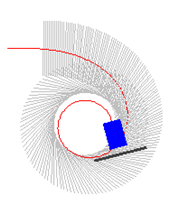
\includegraphics[width=0.3\textwidth]{3-ConceptDesign/Detector_Coverage1.png}}
& \subfloat[Trial 2]{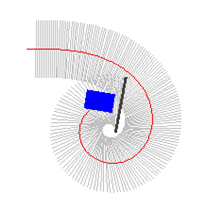
\includegraphics[width=0.3\textwidth]{3-ConceptDesign/Detector_Coverage2.png}}
& \subfloat[Trial 3]{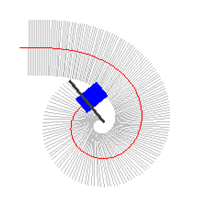
\includegraphics[width=0.3\textwidth]{3-ConceptDesign/Detector_Coverage3.png}}\\
\end{tabular}}
\caption{Sensor coverage simulations} 
\figlabel{turnCoverage}
\end{figure}

\begin{itemize}
\item \textbf{Trial 1}: In first trial, represented in \Figref{turnCoverage} (a), front wheel steering is used with the sensor mount in front of the platform. The turning wheels are 1.5 metres in front of the focal point of the turn, and the sensor array is 0.5 metres in front of the turning wheels. It is evident from the figure that the coverage area does not form a tight loop, and that this area does not include the path of the vehicle. This is critical as it will mean the quad bike will be passing over ground that has not been scanned by the sensors.
\item \textbf{Trial 2}: In the second trial, represented in \Figref{turnCoverage}(b), rear wheel steering is used (i.e. the quad bike is using front wheel steering in reverse) with the sensor mount at the front of the platform relative to the direction of travel (i.e. to the rear relative to the actual quad bike geometry). The turning wheels are 1.5 metres behind the focal point of the turn, and the sensor array is placed 0.5 metres in front of the focal axle. This trial shows a much tighter scanning loop than the previous test, and the path of the quad bike is entirely within the scanned area, which is the ideal case.
\item \textbf{Trial 3}: The third trial, represented in \Figref{turnCoverage} (c), shows front wheel steering with the sensor mount placed behind the front wheels. The turning wheels are 1.5 metres in front of the focal axle as in Trial 1, but the sensing array is 1.5 metres behind the turning wheels, or between the two axles of the vehicle. Under this arrangement, an identical scanning path to Trial 2 is achieved using front-wheel steering, however this is not very useful since the wheels will pass over the region to be scanned before sensors.
\end{itemize}

This result can be demonstrated theoretically by using the geometric bicycle model \parencite{snider2009}. Referring to \Figref{geometricBicycleModel}, the turning radius of the rear wheel is $R$ and the turning radius of the front wheel is $\sqrt{R^2 + L^2}$, which is greater than $R$. If the sensor array was some distance $q$ in front of the front wheels, its turning radius would be $\sqrt{R^2 + [L+q]^2}$, greater yet again. However, if the sensing array was an equal distance $q$ behind the rear wheels (or front wheels if this was a rear steering arrangement) then the turning radius of the sensors would be $\sqrt{R^2 + q^2}$. From this it can be seen that to minimise the effective turning radius then $q$ should be minimised, i.e. rear wheel steering should be used. To achieve this, the sensor arrays will be mounted at the rear of the quad bike, which will be driven in reverse. 
\nomenclature[S]{$q$}{Sensor array distance from turning wheels}%

\subsection{Initial designs}
Knowing the basic sensor requirements, the selected material for the mount, and the mounting location on the quad bike, preliminary designs for sensor mount were developed. 

There are three support points at the rear of the quad bike to which the mount can be attached, a tow hitch near the rear axle, and two metal brackets beneath the rear tray. The tow hitch has a level surface and is capable of supporting a vertical load of 14 kg, which means that a cantilever beam could be mounted on the tow hitch, but it's weight would be limited. To fix this, diagonal support braces can be used, attached to the two metal brackets. Based on this geometry, a basic design for the sensor mount is shown in \Figref{basic}

\begin{figure}[ht]
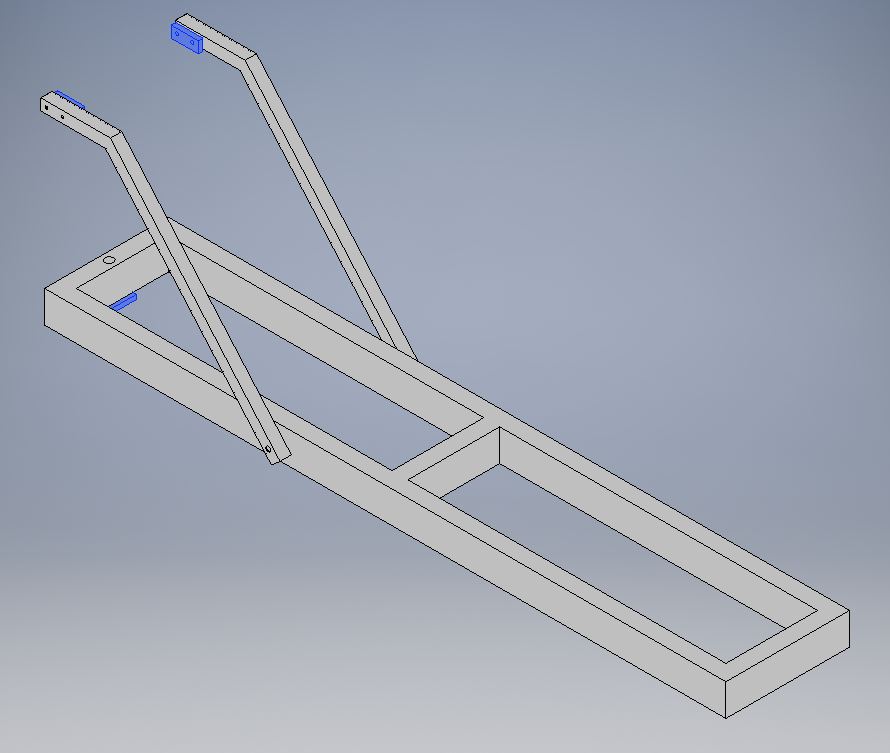
\includegraphics[width=.6\textwidth]{3-ConceptDesign/basic.PNG}
\centering
\caption{Basic sensor mount with support points in blue}
\figlabel{basic}
\end{figure}

A multi-beam structure is used rather than a single cantilever in order to reduce mass and improve torsional rigidity. The main beam rests on the tow hitch, and is made of wood. The two diagonal supports could also be made of wood, however metal supports provides a more rigid frame. The total length of the frame is 1.5 m, which allows enough length for the metal detector and GPR to be mounted with the required minimum proximity. 

\textcolor{red}{Add details about the perspex case for the MD, different concepts for mounting the MD, design for GPR attachment. Nylon rods allow height of MD to be adjusted, same with a telescopic rod for the GPR. Wooden supports add torsional stiffness, preventing MD from moving as much compared to nylon rods alone. }

% \begin{figure}[ht]
% 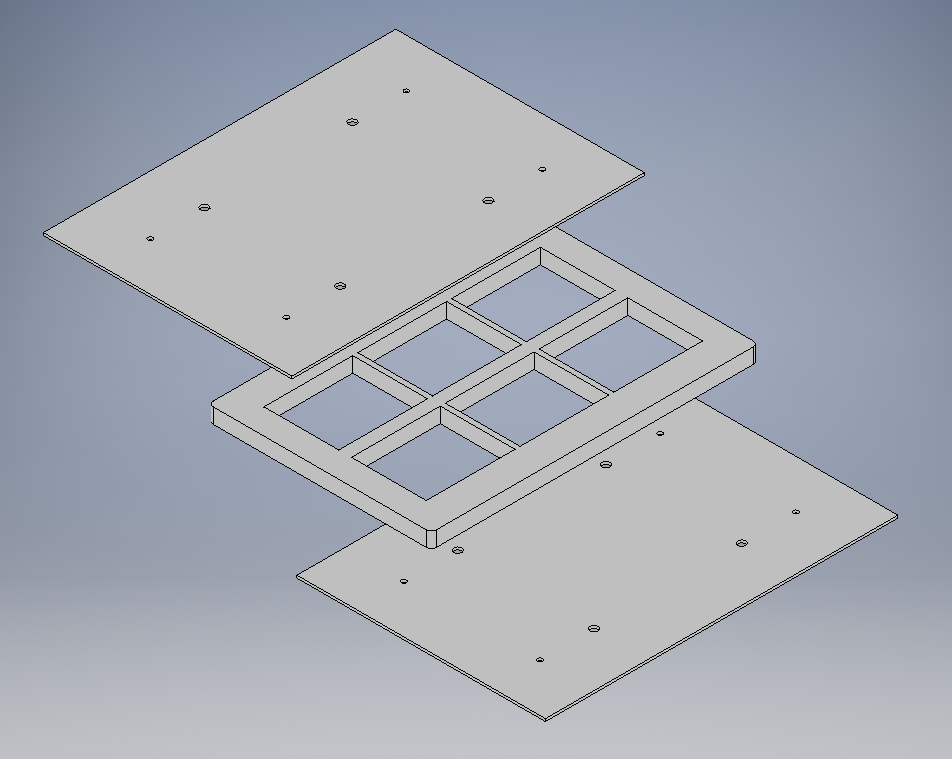
\includegraphics[width=.5\textwidth]{3-ConceptDesign/MD.PNG}
% \centering
% \caption{Metal detector with Perspex covers}
% \figlabel{MD}
% \end{figure}

% \begin{figure}[ht]
% \centerline{
% \begin{tabular}{cc}
% \subfloat[]{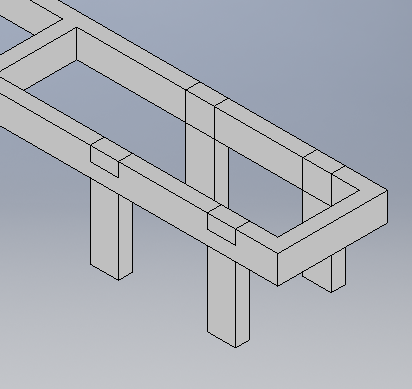
\includegraphics[width=0.4\textwidth]{3-ConceptDesign/square.PNG}}
% & \subfloat[]{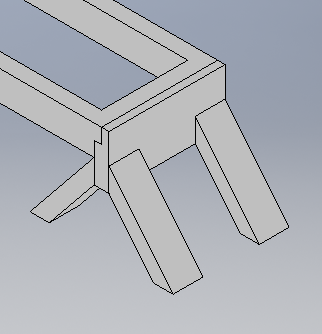
\includegraphics[width=0.4\textwidth]{3-ConceptDesign/triangle.PNG}}\\
% & \subfloat[]{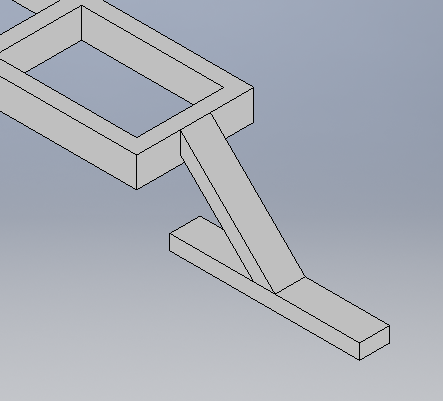
\includegraphics[width=0.4\textwidth]{3-ConceptDesign/cantilever.png}}\\
% \end{tabular}}
% \caption{Concepts for attaching the metal detector the the sensor mount} 
% \figlabel{MDdesigns}
% \end{figure}

\section{Subsystem integration}
\textcolor{red}{Introduction for the section}

\seclabel{conceptprojectdesign}

% \subsection{Electronics}
% As a major component of the project is advanced signal processing in real time, significant computational capabilities will be required on the quad bike. In addition to signal processing, other platform software systems such as vehicle control and telemetry will also be running. To achieve this without requiring multiple discrete hardware components (which would require communications input/output (I/O) interfaces to share data), a single hardware system capable of executing multiple threads simultaneously and asynchronously is required on the vehicle. The hardware system executing the signal processing software must also be capable of reading sensory input from USB devices, as this is the communications format available on the SIRO-PULSE II GPR unit. 
% \nomenclature[A]{I/O}{Input/Output}% 

% A second major component of the project is the automation of the quad bike, requiring software control over a series of actuators and sensors. To provide the greatest fidelity of control over the vehicle, the electronics hardware used to interface with the actuators and sensors must be capable of reading and writing to low-level I/O devices quickly and with minimal latency or overhead. 

% \begin{itemize}
% \item \textbf{Bespoke Electronics}\\
% Bespoke electronic equipment has the capacity to allow incredibly fast access to I/O devices through the use of task-specific commercial off-the-shelf (COTS) chips. However, the time consumption and expense of planning an entirely hardware-driven control system for anything more than trivial data handling is inappropriate for this project. The inability to prototype as with software means that the ability to test and then revisit a solution is not possible, and a hardware/purely electronics driven system is not capable of general purpose processing. Therefore, this is not a realistic option for achieving the project aims.
% \nomenclature[A]{COTS}{Commercial off-the-shelf}% 
% \item \textbf{Microcontrollers}\\
% Microcontrollers have become the de facto standard for small to medium software-based projects which require access to physical sensors and actuators, due to their readily available access to low level I/O. Microcontrollers supporting common languages such as C++ and Java allow easy development and rapid prototyping, though the inability to easily connect debugging equipment or generate test output slows the development process. Microcontrollers are inexpensive and provide high I/O availability but at the cost of limited processing power. The low-level nature of microcontrollers means that desirable features like hardware interrupts are exposed to and accessible by developers. 
% \item \textbf{Desktop computing equipment/Laptop} \\
% Conventional desktop computing equipment is the fastest general purpose computing hardware that will be available to the project. In addition to having the greatest computing power, it has the highest ability to support prototyping and allows for rapid software development with readily accessible software generation and debugging tools. The drawback of this higher-level computing platform is the reduced accessibility of low-level I/O devices, and the amount of computing overhead caused by operating system processes. Operations that require fast I/O access may be hampered by the inability to ensure thread availability, and so for robust operation this may require buffering to a secondary, lower level device.
% \end{itemize}

% None of the individual items presented allow for the full range of requirements of this project. As a result, the general concept for the hardware arrangement to execute the software systems is shown below in \Figref{hardwareLayout}.
% % is this figure text fucking big enough maziar??
% \begin{figure}[ht]
% 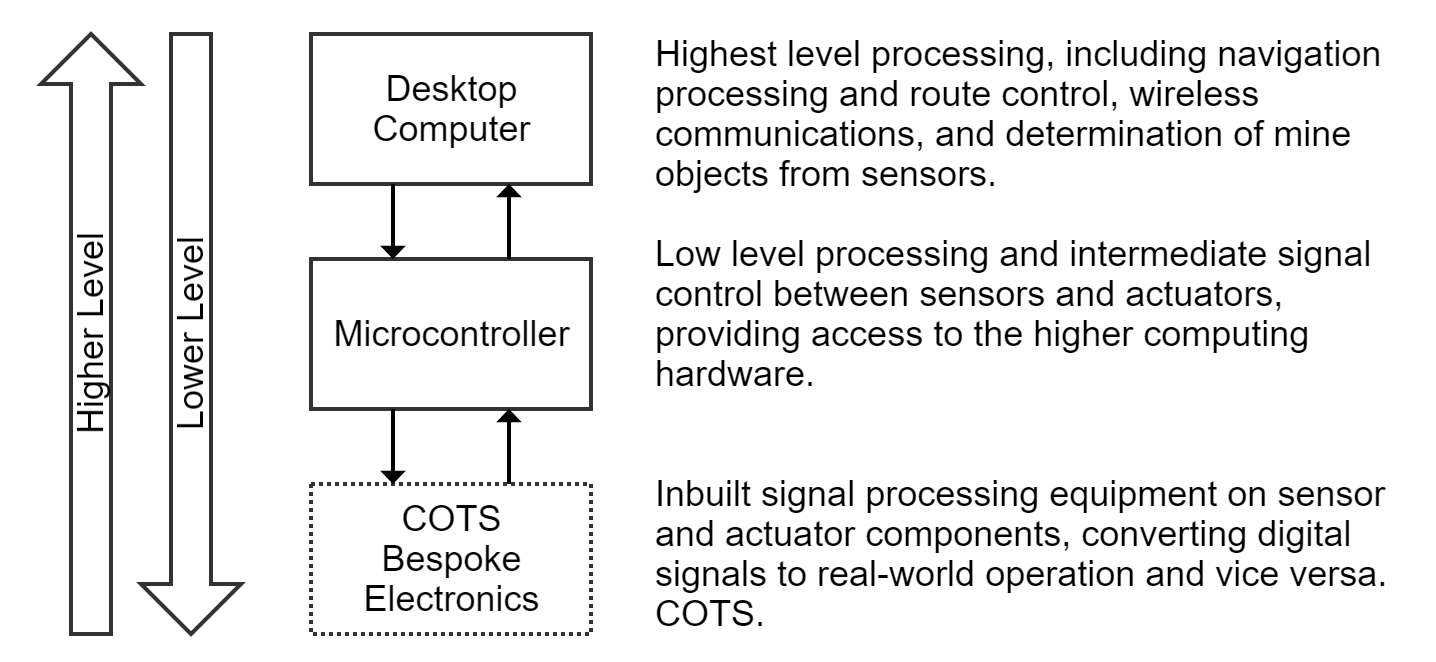
\includegraphics[width = \textwidth]{3-ConceptDesign/electronics.png}
% \centering
% \caption{Conceptual hardware layout} \figlabel{hardwareLayout}
% \end{figure}

% Under this system, the project will use standard desktop computing equipment for the bulk of the software, to make use of its superior processing power and the rapid development it allows. This device will be the data handler and processor, and act as the 'central' software location for the project. Sensors and actuators that require low level I/O access will be connected to a secondary microcontroller, which will act independently to buffer inputs and outputs of the system, which can then be communicated to the primary computer over a serial communications connection. The project will not aim to develop any custom electronics boards and handle all signal amplification or processing in software.

\subsection{Software architecture}
The autonomous quad bike will be used as the platform on which the sensor mount and software subsytems will operate. To achieve the framework for overall automation of the platform the integration of the actuator electronics, navigation, sensors, signal processing and operator device is required. This framework is completed through the Central Hub as shown in \Figref{central} where dotted lines indicate implementations of the interfaces. The Central Hub will combine and read all the relevant processes and transmit the required information to the operator device. This enables all processes to be completed in parallel on independent threads, satisfying the deliverables as defined in \secref{primary}.

\begin{figure}[ht]
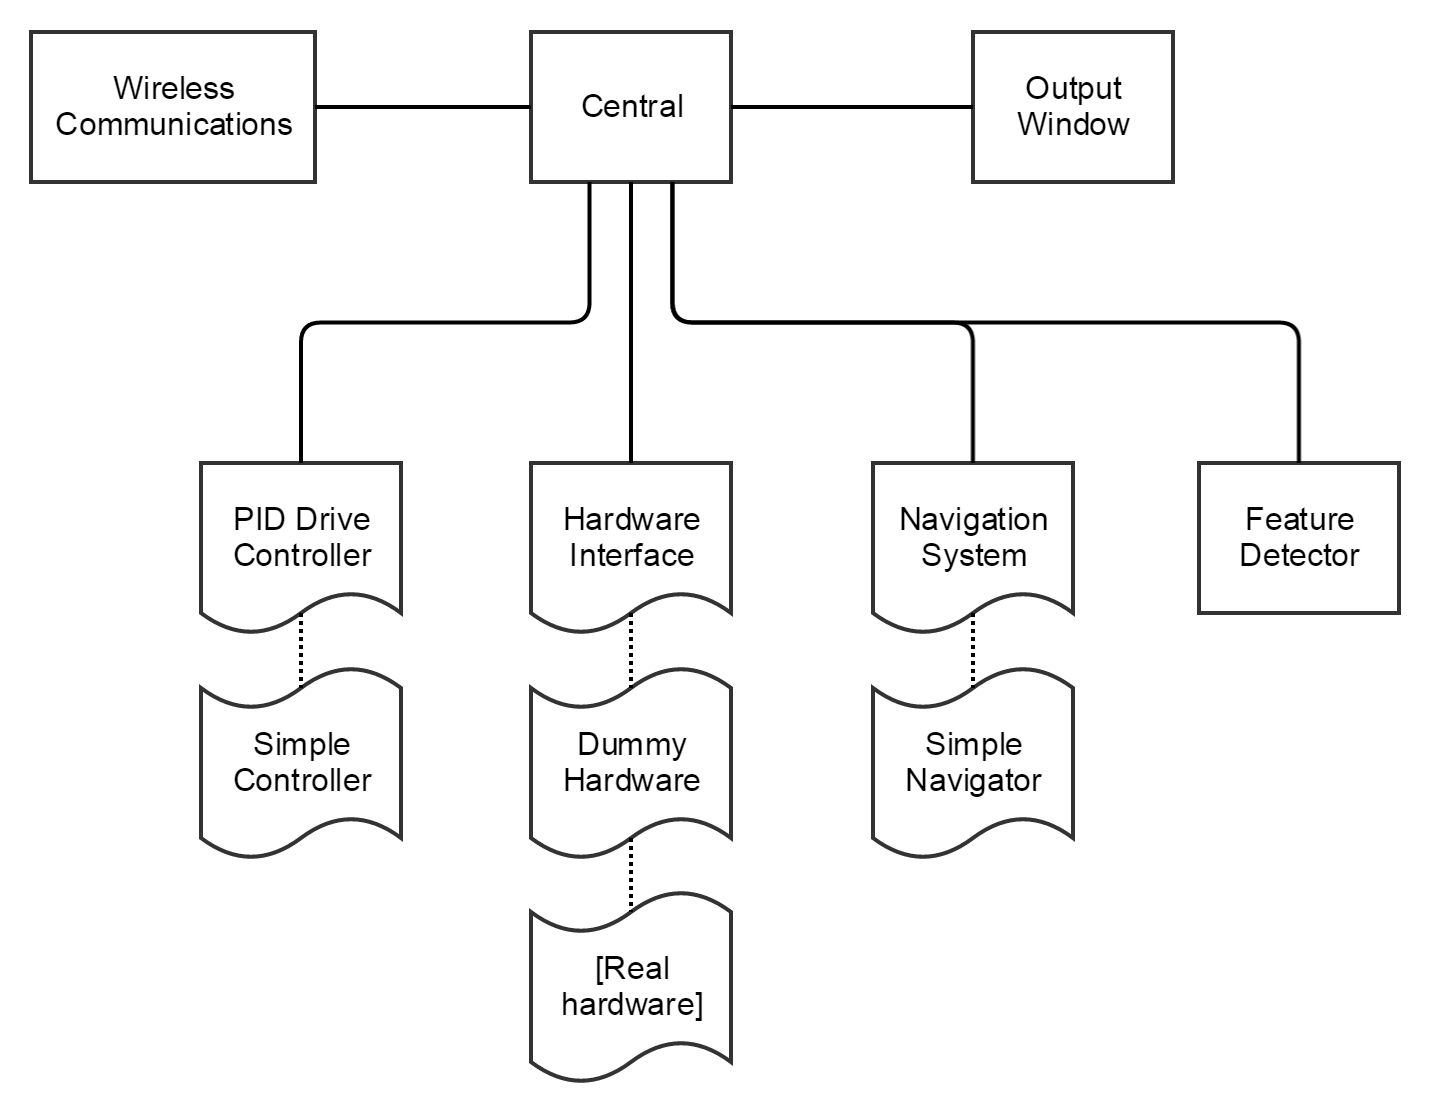
\includegraphics[width=\textwidth]{3-ConceptDesign/fyp_structure.png}
\centering
\caption{Integration of automation, navigation, sensors and signal processing} 
\figlabel{central}
\end{figure}

The mine detection system as a whole requires at minimum two control devices: the control system on the remote platform, and the control device held by a remote operator. The various subsystems involved in the software design were considered when selecting these control devices, and the decision was made to place the majority of software base on the on the remote platform. Having the majority of software systems physically residing on the remote platform allows the vehicle to remain in control of all systems in the event of a communications loss, meaning that necessary actions to stop the vehicle can be made if a severance of communications is detected. Under this scheme, the operator device would act only as a remote terminal to relay data to the central processing system.

\subsection{Electronics}
A conventional PC running a Windows XP operating system was chosen for the primary control device on the remote platform, as this was a requirement to interface with the supplied GPR and metal detector. The PC also allowed for maximum ease of development under a familiar operating environmental, and provided tools for fast debugging of code.

The control device on the remote platform needed to provide low level I/O to support the sensors and actuators controlling the motion of the quad bike. This functionality is available through a conventional PC, however can be difficult to configure correctly and suffers from delay and buffering issues caused by thread switching. The options available were to retain the PC as the sole electronic controller, or to push the control of low level sensors and actuators to a microcontroller which was better suited to the task. The microcontroller was selected due to its low cost, high I/O flexibility and the ability to manage I/O at a consistent cycle rate. 


\subsection{Communications}
Communications between electronics systems inevitably introduces latency in signals and so the relationships between electronics systems were chosen to minimise the amount of data that was required to be transmitted. This also minimises the possibility of the communications channel becoming saturated and blocking the transmission of important time critical signals, such as an emergency stop. Where possible, data will be retained within the bounds of a single controller and only transferred when absolutely required. The major communications interfaces in the control system are detailed in the diagram below.

\textcolor{red}{Xx insert image – low level I/O to Arduino (inc GPS and IMU). Smart motor Serial to Arduino. Arduino Serial to PC. PC to tablet Wifi. XXXxxX}

An example of our minimal communications strategy is evident from the above figure. The output from the GPS unit is a series of registers which is reported to the Arduino at a rate of approximately 10 Hz. Some degree of processing is required to translate this block of data into a geographic position, which can be represented by only two numbers. To reduce communications overhead, the Arduino is responsible for performing this calculation and will only report the position to the PC when explicitly requested to. This limits the volume of data required to be transmitted, and can limit the rate at which the transmission is sent. As the PC is the central unit for all other systems, the PC also maintains control over all of the communications interfaces and is responsible for initiating all communication traffic.

\end{document}

















